\documentclass[10pt,twocolumn]{article} 

% required packages for Oxy Comps style
\usepackage{oxycomps} % the main oxycomps style file
\usepackage{times} % use Times as the default font
\usepackage[style=numeric,sorting=nyt]{biblatex} % format the bibliography nicely

\usepackage{amsfonts} % provides many math symbols/fonts
\usepackage{listings} % provides the lstlisting environment
\usepackage{amssymb} % provides many math symbols/fonts
\usepackage{graphicx} % allows insertion of grpahics
\usepackage{hyperref} % creates links within the page and to URLs
\usepackage{url} % formats URLs properly
\usepackage{verbatim} % provides the comment environment
\usepackage{xpatch} % used to patch \textcite

\bibliography{references}
\DeclareNameAlias{default}{last-first}

\xpatchbibmacro{textcite}
  {\printnames{labelname}}
  {\printnames{labelname} (\printfield{year})}
  {}
  {}

\pdfinfo{
    /Title (Writing Your Oxy CS Comps Paper in LaTeX)
    /Author (Maryo Botros)
}

\title{SLAM}

\author{Maryo Botros}
\affiliation{Occidental College}
\email{mbotros@oxy.edu}

\begin{document}

\maketitle

\begin{abstract}
    Abstract
\end{abstract}

\section{Problem Context}

Robotics boasts a significant benefit in accomplishing repeatable, tedious, or menial tasks at high effieciencies and with great resource utilization. Robots can increase relative productivity and decrease resource and energy consumption by multiple orders of magnitude for processes. They can also offer high-precision with limited human oversight for the tasks they are designed for. The real benefit of robotics comes in where robotics can serve as a substitute for human labor, more specifically, human labor that can potentially put humans in harm's way and some of the best robots for accomplishing this task are vehicles that can navigate autonomously. An example of one of these tasks includes using the robot to enter a building on fire to search for and potentially rescue people. Another application can be for military applications, such as reconnaissance. These are just two of the many possible applications of autonomous vehicles. These robots are very useful, but getting them to accomplish the task of being autonomous does not come easily.

The problem is that getting a robot to navigate any environment is challenging and is rooted in uncertainty. There are two things a robot must be able to do to autonomously navigate. It must understand the map of its environment, which is known as mapping. It must also know where it is on that map, which is known as localization. The problem is that in order for the robot to know where it is on the map, it must first understand the map, but in order for it to understand the map, it must first understand where it is on the map. This poses a major challenge because there are conflicting dependent conditions. The solution to this problem is doing both the mapping and the localization at the same time and this process is known as SLAM. SLAM means simultaneous localization and mapping and it's the method for getting a robot to autonomously navigate its environment. SLAM is still an open problem and new ways of solving the problems of navigation are still being researched constantly.


\section{Technical Background}

A few of the problems involved with navigation that will be covered in this project are localization, searching for the goal location, planning a path to the goal location, covering an entire area, and SLAM.

One of the ways localization is accomplished for robots is using odometry or the distance the robot has traveled. Shaft encoders are the sensors used for odometry. One problem with this however is that the farther the robot has traveled, the more inaccurate the odometry will be because measurements of the physical environment are unavoidable.

Search and path planning involves finding a path from the robot’s current location, to the destination. Two things that the robot would have to know to do this are what the map looks like as well as where it is on that map (localization). It must know both of these within a common frame of reference. There are typically many different paths for getting to the destination from the starting point. Graphs with nodes and lines are usually used for modeling a map. The criterion for the optimal path can be safety or distance for example and finding the optimal path may require searching all paths. A maze is one of the best ways of testing a robot’s ability to get to a goal location. One of the methods for solving a maze can be programming the robot to follow one of the walls of the maze. This method will work but it is the naive solution and is not the most efficient as it can take a long time, depending on the complexity of the maze. A much more optimal solution for solving a maze is by using a depth-first search approach, where the robot will keep track of each path option in the maze as a node and it will go down all the nodes along a single path first before it backtracks and then goes along a different path until it has found the exit to the maze. The way this would be executed is by using a graph data structure, like the one in Figure 1. The graph is a good model for the maze. Each junction in the maze is recorded as a node in the graph model. There are several other algorithms besides the depth-first search for navigating the maze, such as a breadth-first search, but this is one of the most efficient solutions.

Coverage is a problem that certain robots such as robot vacuums need to be able to efficiently solve. If the robot has a map available to it, the problem of coverage becomes a lot easier. In this case, the robot would need all navigable spaces on the map until the whole map is covered, or the robot has accomplished its designated goal, such as searching for an object or reaching a destination. If the robot does not have a map available, there are certain heuristics it can follow such as following a continuous boundary like a wall. 

SLAM is a difficult problem because it requires the robot to do two ongoing processes. One thing that makes SLAM difficult is the data association problem, or basically, the problem that certain locations on the map may look similar, which leads to ambiguity while the robot is navigating. When the robot is constructing a map, if it sees a particular chair at one location and then sees a similar chair at a different location, it would have a hard time distinguishing the two \textcite{Mataric2008TheRoboticsPrimer}.

  \begin{figure}
    \centering
    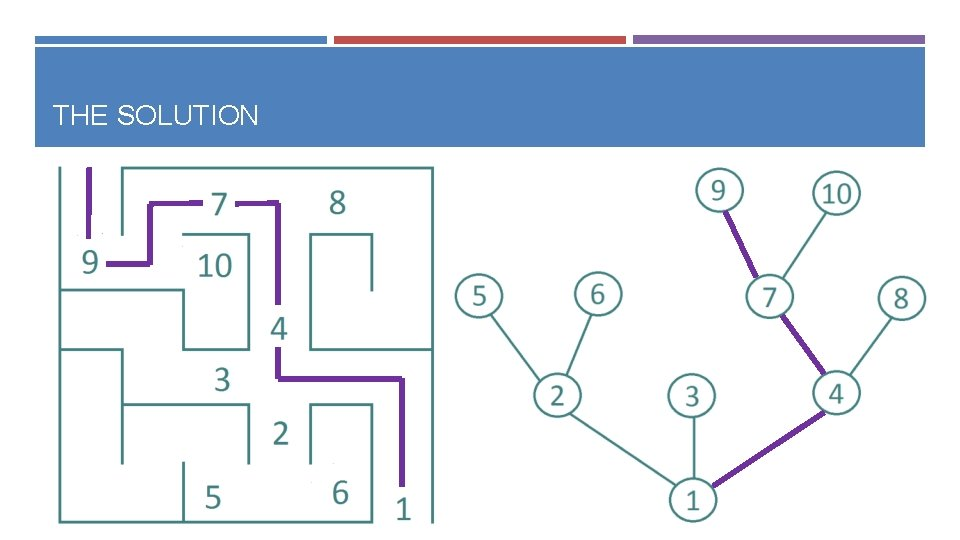
\includegraphics[width=.95\linewidth]{graph.jpg}
    \caption{
        Maze and graph}
    \label{fig:Figure1}
\end{figure}
  

\section{Prior Work}
As stated earlier, SLAM is still an open problem that is being researched. However, there is already a myriad of already-existing research that sheds light on the greatest advancements in the subject area. Although there are many solutions for solving the problems with SLAM, there are always arising obstacles depending on the application.

In 2018, Geo Week News posted an online article explaining how SLAM is too power-intensive and too slow, which renders it useless for faster robots, such as fast drones. For small drones, SLAM is so power-intensive that there is not enough onboard processing capacity to handle the complex calculations. To combat this issue a new method called NanoMap is being used. Created by researchers at MIT’s Computer Science and Artificial Intelligence Lab (CSAIL), NanoMap uses 3D depth sensors to perform navigation fast, enabling autonomous drones to reach high speeds of up to 20 mph. Unlike SLAM, NanoMap does not generate a holistic map of the environment and uses some uncertainty when it comes to localization. It uses its depth sensors to gather 2D snapshots of its environment and then stores those snapshots. So when it reaches a location, it reaches into its memory and tries to figure out where it is based on how closely related one of the images is to what it is currently seeing \textcite{GeoWeekNewsStaff2018NanoMap}. This is not an ideal approach as there is just too much uncertainty involved, but it does reveal a shortcut that could potentially be useful if it could somehow be combined with SLAM.

Madeline Shiappa, a PhD student at UCF sheds some light on learning methods for SLAM, including the Kalman Filter, which is the most common learning method for SLAM. The Kalman Filter is a type of Bayes Filter used for state estimation It is a recursive algorithm that makes a prediction then goes back and corrects the prediction over time. In order to correct the prediction, sensors are necessary. There are two categories of sensors: proprioceptive and exteroceptive. The exteroceptive sensors are the ones that collect information from the robot’s environment such as if there’s an object in front of the robot and some of these sensors include sonar, range lasers, and cameras. Proprioceptive sensors collect information that is internal to the robot, such as its position and acceleration, using encoders, gyroscopes, and accelerometers. The combination of these two types of sensors produces a very effective feedback system. Madeline Shiappa also acknowledges the computational complexity as a limitation of SLAM. The more dimension in states and measurements, the more intractable the calculations become, which creates a tradeoff between accuracy and complexity \textcite{Schiappa2019HowDoesAutonomous}.
\subsection{Goals}

\subsection{Audience}

\subsection{Requirements}

\section{Sections of the Oxy CS Comps Paper}

\subsection{Introduction and Background}


\subsection{Prior Work}

\subsection{Methods}

\subsection{Evaluation}

\subsection{Ethical Considerations}

\subsection{Limitations, Future Work, and Conclusion}

\subsection{Appendices}

\section{Conclusion}

\printbibliography 

\end{document}
